\documentclass[8pt,a4paper,compress]{beamer}

\usepackage{/home/siyer/lib/slides}

\title{Your First Program}
\date{}

\begin{document}
\begin{frame}
\vfill
\titlepage
\end{frame}

\begin{frame}
\frametitle{Outline}
\tableofcontents
\end{frame}

\section{Programming in Python}
\begin{frame}[fragile]
\pause

\begin{minipage}{200pt}
Our programming environment
\begin{itemize}
\item Python programming language  
\item IDLE, a simple integrated development environment (IDE)
\item Terminal
\item Input and output libraries from the authors of the IPP text \end{itemize}
\end{minipage}%
\begin{minipage}{100pt}
\begin{center}
\visible<2->{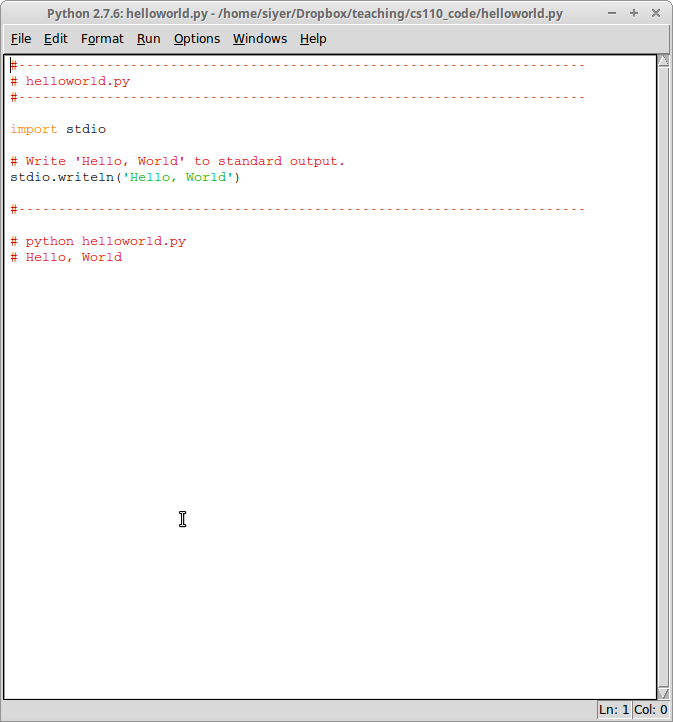
\includegraphics[scale=0.16]{figures/idle.png}}

\smallskip

\tiny IDLE

\smallskip

\visible<2->{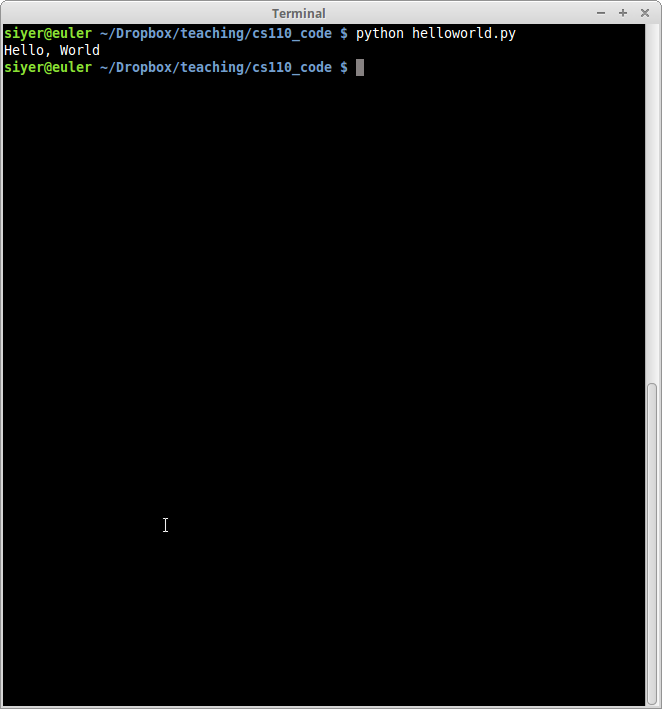
\includegraphics[scale=0.16]{figures/terminal.png}}

\smallskip

\tiny Terminal
\end{center}
\end{minipage}
\end{frame}

\begin{frame}[fragile]
\pause

To program in Python
\begin{itemize}
\item Compose a program by typing it into a file named, say, \lstinline{helloworld.py}
\item Run (or execute) the program by typing \lstinline{python helloworld.py} in the terminal window
\end{itemize}

\begin{center}
\begin{tikzpicture}
\begin{scope}[->,xshift=-7.5cm,yshift=-5cm,thin,
	   node distance=2.0cm,on grid,>=stealth,
  	   block1/.style={rectangle,draw,align=center},
	   block2/.style={rectangle,align=center}]
\node [block1] (1) {editor \\ (IDLE)};
\node [block2] (2) [right=of 1] {\lstinline$helloworld.py$};
\node [block1] (3) [right=of 2] {compiler/ \\ interpreter \\ (\lstinline$python$)};
\node [block2] (4) [right=of 3] {\lstinline$Hello, World$};
\path (1) edge node [above] {} (2);
\path (2) edge node [above] {} (3);
\path (3) edge node [above] {} (4);
\end{scope}
\end{tikzpicture}
\end{center}
\end{frame}

\begin{frame}[fragile]
\pause

\begin{framed}
\tiny helloworld.py: Write 'Hello, World' to standard output.
\end{framed}

\begin{lstlisting}[language=Python,numbers=left]
import stdio

# Write 'Hello, World' to standard output.
stdio.writeln('Hello, World')
\end{lstlisting}

\pause

\begin{lstlisting}[language={}]
$ python helloworld.py 
Hello, World
\end{lstlisting}

\pause
\bigskip

Anatomy of \lstinline{helloworld.py}
\begin{itemize}
\item The first line is a statement that tells Python that you intend to use features defined in the \lstinline{stdio} module
 
\item The second line is a blank line; Python ignores blank lines; programmers use them to separate logical blocks of code

\item The third line is a comment; Python ignores comments; they are only for human readers of the program

\item The fourth line is a statement that calls the \lstinline{stdio.writeln()} function to write the given text to the terminal; This is called ``writing to standard output''
\end{itemize}
\end{frame}

\begin{frame}[fragile]
\pause

Errors (aka bugs) are the bane of a programmer's existence

\pause
\bigskip

Compile-time errors are raised when Python compiles a program

\pause
\bigskip

For example, if we don't include the right parenthesis in line four of \lstinline{helloworld.py}

\pause
\bigskip

Run-time errors are raised when Python interprets a program

\pause
\bigskip

For example, if we forget to import the \lstinline{stdio} module in \lstinline{helloworld.py}
\end{frame}

\section{Input and Output}
\begin{frame}[fragile]
\pause

Bird's-eye view of a Python program
\begin{center}
\begin{tikzpicture}
\begin{scope}[->,xshift=-7.5cm,yshift=-5cm,thin,
	   node distance=2cm,on grid,>=stealth,
  	   block1/.style={rectangle,draw,align=center},
	   block2/.style={rectangle,align=center}]
\node [block2] (1) {input};
\node [block1] (2) [right=of 1] {\lstinline$my_program.py$};
\node [block2] (3) [right=of 2] {output};
\path (1) edge node [above] {} (2);
\path (2) edge node [above] {} (3);
\end{scope}
\end{tikzpicture}
\end{center}
\begin{itemize}
\item Input types: command-line arguments, standard input, file input
\item Output types: standard output, file output, graphical output, audio output
\end{itemize}
\end{frame}

\begin{frame}[fragile]
\pause

Command-line arguments are the inputs we list after a program name when we run the program

\begin{lstlisting}[language={}]
$ python my_program.py arg_1 arg_2 ... arg_n
\end{lstlisting}

\pause
\bigskip

The command-line arguments can be accessed within a program, such as \lstinline{my_program.py} above, via the array (aka list) \lstinline{sys.argv}\footnote{The \lstinline{sys} module provides access to variables and functions that interact with the Python interpreter}  as \lstinline{sys.argv[1]}, \lstinline{sys.argv[2]}, $\dots$, \lstinline{sys.argv[n]}

\pause
\bigskip

The name of the program (\lstinline{my_program.py}) is stored in \lstinline{sys.argv[0]} 
\end{frame}

\begin{frame}[fragile]
\pause

\begin{framed}
\tiny useargument.py: Accept a name as a command-line argument. Write a message containing that name to standard output.
\end{framed}

\begin{lstlisting}[language=Python]
import stdio
import sys

stdio.write('Hi, ')
stdio.write(sys.argv[1])
stdio.writeln('. How are you?')
\end{lstlisting}

\pause
\begin{lstlisting}[language={}]
$ python useargument.py Alice
Hi, Alice. How are you?
$ python useargument.py Bob
Hi, Bob. How are you?
$ python useargument.py Carol
Hi, Carol. How are you?
\end{lstlisting}
\end{frame}
\end{document}
